% !TEX encoding = UTF-8 Unicode
%!TEX root = main.tex
% !TEX spellcheck = en-US
%%=========================================


%%%%%%%%%%%%%%%%%%%%%%%%%%%%%%%%%%%%%%%%%%%%%%%%%%%%%%%%%%%%%%%%%%%%%%%%%%%%%%%%%%%
\chapter{Design and Implementation}
\label{ch:design_implementation}

This chapter explains the details in design and the implementation of the core library features of ProXC. The presented design and implementation is for a single\hyp{}core implementation. 

The library will be written in C, with standard GNU99 dialect. Any details regarding the C programming language will not be explained. Refer to a C reference (e.g. \citet{k&r}) for more detailed descriptions.   


%%%%%%%%%%%%%%%%%%%%%%%%%
\subsection*{Terminology}

From here on, the term ``\textit{process}'' means a single user\hyp{}thread meant to run sequential C code from a C program. The term ``\textit{parent scheduler}'' in the context of a process means the scheduler which the process is designated to, i.e. both reside on the same kernel\hyp{}thread. The term ``\textit{running process}'' corresponds to the process that is currently executed on a given kernel\hyp{}thread, given that the scheduler has resumed a process. The term ``\textit{ownership}'' in the context of a scheduler owning a process means the scheduler is a parent scheduler to the process. The term ``\textit{root process}'' in the context of composite processes means the process that defined and spawned the composite process.


%%%%%%%%%%%%%%%%%%%%%%%%%%%%%%%%%%%%%%%%%%%%%%%%%%%%%%%%%%%%%%%%%%%%%%%%%%%%%%%%%%%
\section{Run\hyp{}Time System}
\label{sec:run-time_system}

The run\hyp{}time system of ProXC forms the foundation for how the library is able to implement a CSP model in C. Some sort of a threading model has to be implemented when implementing a CSP model for programming, which is discussed in Section \ref{sec:concurrency_vs_parallelism}, \ref{sec:threading_models} and \ref{sec:csp}. The choice of threading model is an important choice regarding performance, and is analysed in \citet[chapter 1]{c++csp2}. The paper reasons that the context switch time between threads is the major factor in performance, and argues that the hybrid model would be the best choice for the CSP library. For a multi\hyp{}core implementation, a hybrid model would be the preferred choice. However, as this is a single\hyp{}core implementation, a user\hyp{}thread model will be used in this implementation.

The core of the run\hyp{}time system is the scheduler, which controls the flow of execution from a collection of processes. In the threading model, each kernel\hyp{}thread has a permanent corresponding scheduler, scheduling multiple processes on said kernel\hyp{}thread. However, it is important to understand that the scheduler itself is a user\hyp{}thread on the kernel\hyp{}thread. Each process is a user\hyp{}thread. The kernel\hyp{}thread executes only one user\hyp{}thread at the time, and the scheduler decides which process is to be resumed by context switching. The context switch only switches between the scheduler and a process context, or vice versa. 

\begin{figure}[h!]
    \centering
    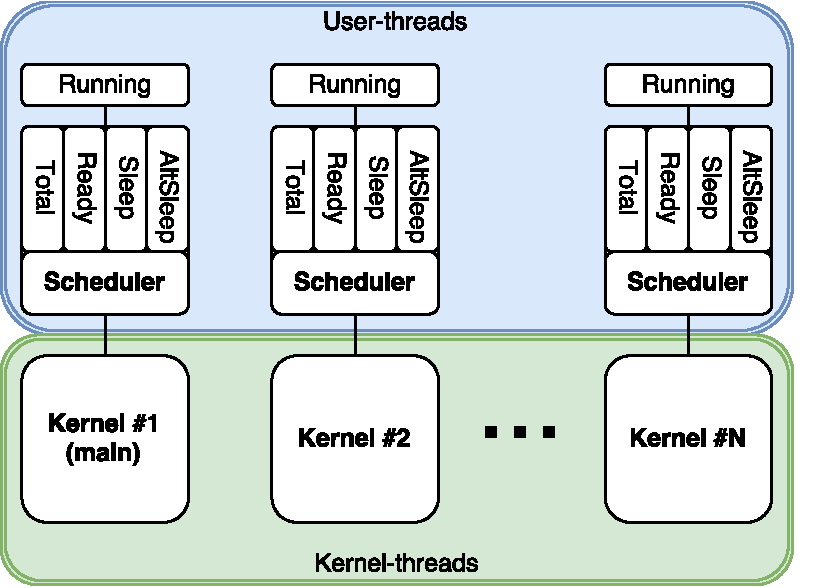
\includegraphics[width=0.6\linewidth]{fig/run-time_system}
    \caption{Overview of the run-time system, with N online processor cores}
    \label{fig:run-time_system}
\end{figure}

When the \texttt{START} procedure is called, the run\hyp{}time system creates and initializes the main process, specified by the programmer. Afterwards, the scheduler is created and initialized. The main process is registered in the scheduler, and the main loop of the scheduler is activated. The scheduler main loop will continue running until one of two thins happen: the main process returns, or the \texttt{EXIT} procedure is called. 


%%%%%%%%%%%%%%%%%%%%%%%%%%%%
\subsection{Data Structures}
\label{subsec:data_structures}

Two types of data structures are used by the run\hyp{}time system: queues and trees. These data structures are not supported in the C standard library, and has to either be implemented or use an existing third\hyp{}party implementation.

For this project, the BSD libc implementations of queues and trees, \texttt{sys/queue.h} \citep{manqueue} and \texttt{sys/tree.h} \citep{mantree}, is used respectively. \texttt{sys/queue.h} implements four types of queues: singly\hyp{}linked lists, singly\hyp{}linked tail queues, lists, and tail queues. \texttt{sys/tree.h} implements two types of trees: red\hyp{}black trees and splay trees. 

These implementations are header\hyp{}only, dependency free, requires no dynamic allocations, and are type\hyp{}safe. This is highly beneficial for the development of the run\hyp{}time system. No dynamic allocations will also lower the run\hyp{}time overhead. 

Tail\hyp{}queues, hereafter called tailq, and red\hyp{}black trees, hereafter called rb\hyp{}tree, will be used in the scheduler implementation. 


%%%%%%%%%%%%%%%%%%%%%%%%%%%%%%%%%%%%%%
\subsection{Thread\hyp{}Local Storage}
\label{subsec:thread-local_storage}

A \textit{thread\hyp{}local storage} (TSD) variable is used in multithreaded programs where a single global variable would be inappropriate. An example of such situations is where a global variable is used to store some internal state of the program. Having multiple threads accessing this global variable could possibly overwrite a previous written value from another thread. TSD solves this by letting the variable be global, but exists only once per thread. 

TSD is used by the run\hyp{}time system to retrieve the scheduler link at any given context, as well as what the current running process is. Picture it like this: whenever a process makes a call to the library, the run\hyp{}time system is invoked. The run\hyp{}time system has no context on which process or which scheduler the call is made from. Using the TSD, the run\hyp{}time system finds which scheduler belongs to this kernel\hyp{}thread, and in turn which process is currently running. With these links, the library call can be processed. 

Since this is a single\hyp{}core implementation, a simple global variable would achieve the same results as a TSD. However, it would not work for a multi\hyp{}processor implementation. So TSD is used for a cleaner, scalable and portable implementation. TSD does however introduce some slight overhead, but is negligible for this project.

TSD is implemented using \texttt{pthread\_key\_t} type, which is a POSIX implementation. The TSD type \texttt{pthread\_key\_t} stores a single variable of type \texttt{void*}. The TSD variable is initialized by the run\hyp{}time system at start up.

Together with the TSD variable, the internal procedure \texttt{scheduler\_self} returns a pointer the corresponding scheduler struct for the given kernel\hyp{}thread. This is only used internally by the run\hyp{}time system, and is invisible to the programmer. The POSIX method \texttt{pthread\_getspecific()} is used to retrieve the actual TSD variable.

\noindent\begin{minipage}{\textwidth}
\begin{lstlisting}[style={CustomC},caption={Procedure to find the scheduler for a given kernel\hyp{}trhead}]
Scheduler* scheduler_self(void) {
    static pthread_key_t key_scheduler;
    return pthread_getspecific(key_scheduler);
}
\end{lstlisting}
\end{minipage}

This can also be used to find the current running process struct, as the scheduler always records which process is currently running. It is called \texttt{process\_self}, and is also an internal procedure for the run\hyp{}time system, just as the \texttt{scheduler\_self} procedure.

\noindent\begin{minipage}{\textwidth}
\begin{lstlisting}[style={CustomC},caption={Procedure to find the current running process}]
Process* process_self(void) {
    return scheduler_self()->running_process;
}
\end{lstlisting}
\end{minipage}


%%%%%%%%%%%%%%%%%%%%%%%%%%%%%%%%
\subsection{Stackful Coroutines}
\label{subsec:stackful_coroutines_impl}

User\hyp{}threads are implemented as coroutines. Each user\hyp{}thread is its own coroutines. There are multiple ways to implement coroutines. Most known approach is using the library routines \texttt{setjmp} and \texttt{longjmp} to provide non\hyp{}local flow between different call frames on the stack. This is however not a portable solution, as jumping down the stack relies on undefined behaviour. The C standard does not specify wheter deallocated stack frames is retained in memory when jumping down the stack. This would break on architectures where deallocated stack frames are deallocated when jumping down the stack.

Another approach is using a duff's device \citep{duffsdevice}, splitting up a process into atomic instructions between scheduling points. This is both portable and does not rely on undefined behaviour. However, the procedure of splitting up and defining the atomic instructions can be difficult to implement. This has usually in existing libraries been implemented using macro magic, which is not favorable for this implementation.

The third approach is stackful coroutines, which is used in this implementation. This allows for fast context switches between coroutines, as they are usually implemented in a few assembly instructions. However, the stack has in most implementations fixed size, which makes stack overflow a potential problem. This is discussed in more detail in Section \ref{sec:fixed_stack}. 


%%%%%%%%%%%%%%%%%%%%%%%%%%%%%%
\subsubsection{Coroutine Implementation}

All relevant code for coroutine implementation are found in files \texttt{context.h} and \texttt{context.c}.

Each coroutine has its own stack and a context. The stack acts as the stack frame of the coroutine execution, and is either allocated on the stack (of the main process) or on the heap. The context is a snapshot of the processor registers at a given execution time, and is stored in a C\hyp{}struct. The snapshot consists of registers that must be preserved by the callee and the program counter. See Section \ref{sec:stackful_coroutines} for a more detailed description for why.

When created, the stack is allocated on the heap. The stack pointer is positioned at the top of the allocated memory, and is 16\hyp{}byte aligned. The return address is stored on the stack. The context structure is initialized, and the process function pointer, stack base pointer and stack pointer is stored in the corresponding registers.

A context switch from a coroutine \textit{c1} to a coroutine \textit{c2} does the following: \textit{c1} invokes a context switch from its own context to the context of \textit{c2}. A snapshot of the processors registers are stored in \textit{c1}'s context struct, and the snapshot stored in \textit{c2}'s context struct is loaded into the processors registers. The program counter is the last register to be loaded, as this triggers the continuation of \textit{c2}. From now on, the processor is executing coroutine \textit{c2}.

Currently, context switching is only implemented for x86\_64 and i386 platforms. The context struct for i386 and x86\_64 is in Listing \ref{lst:ctx_i386} and \ref{lst:ctx_x86_64}, respectively. Note that each register is stored as 32\hyp{}bit or 64\hyp{}bit variables, since i386 is a 32\hyp{}bit platform and x84\_64 is a 64\hyp{}bit platform, and the registers are of such width.

\noindent\begin{minipage}{.45\textwidth}
\begin{lstlisting}[caption={Context struct for i386},style={CustomC},label={lst:ctx_i386}]
struct Context {
    // preserved registers
    uint32_t ebx;  
    uint32_t esi;
    uint32_t edi;
    uint32_t ebp;
    uint32_t esp;
    // program counter
    uint32_t eip;
};
\end{lstlisting}
\end{minipage}\hfill
\begin{minipage}{.45\textwidth}
\begin{lstlisting}[caption={Context struct for x86\_64},style={CustomC},label={lst:ctx_x86_64}]
struct Context {
    // preserved registers
    uint64_t rbx;  
    uint64_t rsp;
    uint64_t rbp;
    uint64_t r12;
    uint64_t r13;
    uint64_t r14;
    uint64_t r15;
    // program counter
    uint64_t rip;
};
\end{lstlisting}
\end{minipage}

The context switching procedure has the following C function prototype.

\begin{lstlisting}[style={CustomC},frame={},numbers=none]
void context_switch(Context *from, Context *to);
\end{lstlisting}

The context switching procedure is however implemented in inline assembly. Direct access to processor registers is not supported in native C. By insert inline assembly into the C program, one can directly access the registers. See Appendix \ref{ch:assembly} for full implementation.


%%%%%%%%%%%%%%%%%%%%%
\subsection{Yielding}
\label{subsec:yielding_impl}

Yielding is used to transfer the flow of control from a running process back to the scheduler. To achieve this, the context of both the running process and the scheduler must be available. Getting either the scheduler pointer or the process pointer is enough, as the scheduler and the process has a pointer to each other. 

For the internal process, calling the \texttt{scheduler\_self} would be sufficient, however there is a overhead penalty of acquiring the TSD variable. The yielding procedure is a frequently called procedure by the run\hyp{}time system, and the overhead would quickly accumulate. A simple optimization would be passing the process pointer if it is already known by the caller, and if not a \texttt{NULL} pointer is passed.

See Listing \ref{lst:yielding_procedure} for both internal and external procedure implementation.

\noindent\begin{minipage}{\textwidth}
\begin{lstlisting}[style={CustomC},caption={Internal and external yielding procedure},label={lst:yielding_procedure}]
// Internal procedure
void process_yield(Process *process) {
    Scheduler *scheduler = NULL;
    if (process == NULL) { // Process struct is not known
        scheduler = scheduler_self();
        process = scheduler->current_process;
    } else { // Process struct is known
        scheduler = process->scheduler;
    }
    context_switch(&process->context, &scheduler->context);
}
// External procedure
void YIELD(void) {
    process_yield(NULL);
}
\end{lstlisting}
\end{minipage}

Note that the external procedure has to call the yielding procedure with NULL as argument, since the process pointer is not available. The internal process will then find what the process pointer is.


%%%%%%%%%%%%%%%%%%%%%%%%%%%%%%%%
\subsection{Descheduling Points}
\label{subsec:descheduling_points}

The ability to express concurrency relies on running processes giving the control of execution back, or yielding, to the scheduler at regular intervals, since the scheduler does not use preemption to regain control. This is done through designated descheduling points, either implicitly defined in library calls, or explicitly defined through the \texttt{YIELD} command.

The following library calls and programming contexts \underline{\smash{will}} result in a yield:

\begin{multicols}{2}
\begin{itemize}[topsep=0em,itemsep=-1em,partopsep=0.5em,parsep=1em]
    \item \texttt{YIELD}
    \item \texttt{EXIT}
    \item \texttt{SLEEP}
    \item \texttt{RUN}
    \item Processes returning
\end{itemize}
\end{multicols}

The following \underline{\smash{may}} result in a yield:

\begin{multicols}{2}
\begin{itemize}[topsep=0em,itemsep=-1em,partopsep=0.5em,parsep=1em]
    \item \texttt{GO}
    \item \texttt{ALT}
    \item \texttt{CHWRITE}
    \item \texttt{CHREAD}
\end{itemize}
\end{multicols}

The following \underline{\smash{will not}} result in a yield:

\begin{multicols}{2}
\begin{itemize}[topsep=0em,itemsep=-1em,partopsep=0.5em,parsep=1em]
    \item \texttt{ARGN}
    \item \texttt{PROC}
    \item \texttt{PAR}
    \item \texttt{SEQ}
    \item \texttt{CHAN\_GUARD}
    \item \texttt{TIME\_GUARD}
    \item \texttt{SKIP\_GUARD}
    \item \texttt{CHOPEN}
    \item \texttt{CHCLOSE}
    \item Normal function calls
    \item Normal functions returning
\end{itemize}
\end{multicols}


%%%%%%%%%%%%%%%%%%%%%%%%%%%%%%%%%%%%%%%%%%%%%%%%%%%%%%%%%%%%%%%%%%%%%%%%%%%%%%%%%%%%%%%%%%%
\section{Scheduler}
\label{sec:scheduler}

The scheduler keeps track of the execution state of a kernel\hyp{}thread. The scheduler knows which process is the main process and keeps track of the current process running. 

As mentioned above, the scheduler runs in its own user\hyp{}thread. It is however important to state that the scheduler does not need to allocate a stack for its user\hyp{}thread, as it uses the user stack in the kernel\hyp{}thread as its own local stack. This is not the case for processes, which is explained in Section \ref{sec:processes}.

Two types of data structures are used in the scheduler. It has two queues: a ready queue and a total queue. It also has two trees: a sleep tree and a alternating guard sleep tree. The ready queue is a queue of processes that are ready to be executed. Processes can be added to the ready queue by any other process, or the scheduler itself. The total queue is the total collection of all processes that are present in the scheduler. The sleep tree is a minimal ordered tree of sleeping processes, where the root node of the tree is the process with the smallest time left sleeping. The alternation sleep tree is the same as the sleep tree, where it contains alternating processes.


%%%%%%%%%%%%%%%%%%%%%%%%%%%%%
\subsection{Scheduler Phases}
\label{subsec:scheduler_phases}

The schedulers main loop has three phases: prologue, context switch, and epilogue. Each phase corresponds to what it does before, under and after a context switch to a process. 

In prologue the scheduler does a termination test, checks if any processes are available, wakes up any timed out processes, and finds next process to resume. The termination test succeeds if either the total queue is empty, or the exit flag is set. Checking the ready queue ensures there are any processes available, and if not, suspends the kernel\hyp{}thread until either a process becomes ready. A process becomes ready by either timing out in the sleep trees, or is added to the ready queue by an another scheduler. When a process is ready, the scheduler checks the sleep trees and adds any processes that has timed out to the ready queue. Lastly, it finds which process from the ready queue to resume.

After prologue, the scheduler now has a process to resume execution to. First, the process is registered as the running process in the scheduler. This is used to retrieve the running process link, described in Section \ref{subsec:thread-local_storage}. Then, the actual context switch to the process happens. From here, the flow of execution in the kernel\hyp{}thread jumps from the scheduler to the context of the process. Whenever the process is descheduled, either through an implicit or explicit descheduling point, the flow of execution is returned to the scheduler, and it resumes as if the function call returned.

In epilogue, the state of the returned process is checked and appropriately handled. Currently only the return states of an unaltered process state or an ended process state is handled. The process is added back to the ready queue, or the process is cleaned up, respectively. If the ended process is the main process, the exit flag in the scheduler is set. Lastly, the running process information is reset, and loops back to prologue.

In Listing \ref{lst:scheduler_main_loop} is the pseudocode of the following phases shown.

It is important to note that when entering epilogue, the state of the returned process is chan\-ged in the context of the process. So even though the scheduler sets the state of the process to running in prologue, the process state can and will be changed when execution is returned to the scheduler. This is of course done by the rune\hyp{}time system, and is invisible to the programmer.

\noindent\begin{minipage}{\textwidth}
\begin{lstlisting}[style=CustomC,caption={Pseudocode for scheduler main loop},label={lst:scheduler_main_loop}]
void scheduler() {
    // Phase 1: Prologue
    while ( termination_test() ) {
        wait_for_readyQ_if_empty();
        check_timedout_processes();
        next_process = find_next_process();
        
        // Phase 2: Context switch
        register_running_process(next_process);
        context_switch(next_process);
        
        // Phase 3: Epilogue
        check_state(next_process);
        reset_running_process();      
    }
    // Here the scheduler exits, and the run-time takes over
}
\end{lstlisting}
\end{minipage}


%%%%%%%%%%%%%%%%%%%%%%%%%%%
\subsection{Scheduler Implementation}

All relevant code for scheduler implementation are found in the following files \texttt{scheduler.h} and \texttt{scheduler.c}.

The scheduler is realized by a scheduler struct with method functions which operates on a given scheduler struct. The scheduler struct type is shown in Listing \ref{lst:scheduler_struct_type}.

The scheduler constructor is called \texttt{scheduler\_create}. When created, the scheduler struct is allocated on the heap. The default stack size for the coroutines is determined, the page size of the memory management unit is stored, and the exit flag is nilled out. The scheduler struct pointer is then registered in the TLS variable. The context of the scheduler and the two tailqs and rb\hyp{}trees are initialized.

The scheduler destructor is called \texttt{scheduler\_free}. When cleaned up, the total queue is iterated over and calls the cleanup procedure for each process. Lastly, the scheduler struct pointer is freed up. 

\noindent\begin{minipage}{\textwidth}
\begin{lstlisting}[style={CustomC},caption={Scheduler struct type},label={lst:scheduler_struct_type}]
struct Scheduler {
    Context context;
    size_t  stack_size;
    size_t  page_size; 
    int     is_exit;
    Process *main_process;
    Process *running_process;
    // queues
    struct ProcessQ totalQ;
    struct ProcessQ readyQ;
    // trees
    struct ProcessRB sleepRB;
    struct PRocessRB altsleepRB;
};
\end{lstlisting}
\end{minipage}

When checking the ready queue and no processes are ready, the kernel\hyp{}thread is suspended by sleeping the minimal expiration time in either sleep or alternation sleep rb\hyp{}tree. The wake\hyp{}up procedure, which checks both sleep rb\hyp{}trees for expired timeouts, are straight forward. However, some slight care has to be taken with the alternation sleep tree. Whenever an sleeping alternation process has expired, the scheduler must check if the process has not already been added to the ready queue by another process. The scheduling policy is currently a FIFO queue on the ready queue. 

Registering the current process is done by setting the next process as current process, and setting the state of that process to \textit{Running}. After this, the process is resumed by context switching. When the context switch returns, one additional action is made. A procedure checking the stack usage of the process will advise the kernel of memory usage if the stack usage exceeds a certain limit. This is to reduce the total memory footprint of the run\hyp{}time system. See Listing \ref{lst:scheduler_registering_context_switch} for reference.

\noindent\begin{minipage}{\textwidth}
\begin{lstlisting}[style={CustomC},caption={Scheduler registering and context switch to running process},label={lst:scheduler_registering_context_switch}]
next_process->state = PROCESS_RUNNING;
scheduler->current_process = next_process;
context_switch(&scheduler->context, &next_process->context);
scheduler->current_process = NULL;
memory_advise(next_process->stack);
\end{lstlisting}
\end{minipage}

During epilogue, the state of the process is checked. This reflects on why the process yielded back to the scheduler. If the process state is \textit{Ready} or \textit{Running}, the process is added back to the ready queue. If the state is \textit{Ended}, the termination condition is checked, the composition tree is re-parsed if the process is part of one, and lastly the process struct is freed. See Listing \ref{lst:process_state_epilogue} for reference.

\noindent\begin{minipage}{\textwidth}
\begin{lstlisting}[style={CustomC},caption={Handling of process state in epilogue},label={lst:process_state_epilogue}]
switch(next_process->state) {
case PROC_RUNNING:
case PROC_READY: // fallthrough
    scheduler_addreadyQ(scheduler, next_process);
    break;
case PROC_ENDED:
    // Determine termination status
    scheduler->is_exit = scheduler->is_exit 
                      || (next_process == scheduler->main_process);
    // 
    composite_parse(next_process->composite_block);
    process_free(next_process);
    break;
case PROC_WAIT:
case PROC_SLEEP: // fallthrough
    // Do nothing
    break;
case ERROR:
    process_error(next_process);
    break;
}
\end{lstlisting}
\end{minipage}

%%%%%%%%%%%%%%%%%%%%%%%%%%%%%%%%%%%%%%%%%%%%%%%%%%%%%%%%%%%%%%%%%%%%%%%%%%%%%%%%%%%%%%%%
\section{Processes}
\label{sec:processes}

A process is a sequential execution of C code. In ProXC, and consequently in C, the sequential code is written as a normal function. The process keeps track of which function to execute and its arguments, the coroutine associated with the process, and the state of the process. The process does also express some notion of ownership, as it acknowledges the parent scheduler is the only scheduler it is assigned to.

The processes and the scheduler are both executed as user\hyp{}threads. This means each user\hyp{}thread has its own stack and context, represented as a coroutine.


%%%%%%%%%%%%%%%%%%%%%%%%%%%
\subsection{Process States}

The process state describes the current state of the process after a yield. In the run\hyp{}time system, the process state is used for a couple of things: informing the scheduler the reason for why the process returned control, and knowing when the process ended. The complete finite state machine of all possible process states and transitions are shown in Figure \ref{fig:process_state_fsm}. 
 
\FloatBarrier

\begin{figure}[h]
    \centering
    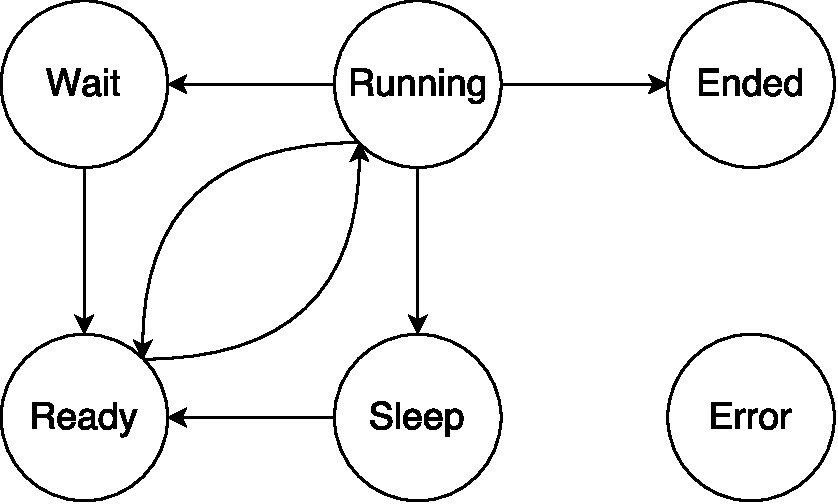
\includegraphics[width=0.6\linewidth]{fig/process_state_fsm}
    \caption{Finite state machine of process states and transitions}
    \label{fig:process_state_fsm}
\end{figure}

\FloatBarrier

The process states describes the following: 
\begin{itemize}[topsep=0em,itemsep=-1em,partopsep=-1em,parsep=1em]
    \item \textbf{Ready state}: the process is in a scheduler's ready queue and is ready to be resumed. 
    \item \textbf{Running state}: the process is currently being executed on a kernel\hyp{}thread, and the\\ scheduler is waiting for the process to return control.
    \item \textbf{Ended state}: the process has reached the end of its sequential code, and can safely\\ be cleaned up.
    \item \textbf{Error state}: the process has entered an unrecoverable state.
    \item \textbf{Wait state}: the process is waiting for an another process to release it. This can happen during synchronization points such as channel communication and alternation without timeout.
    \item \textbf{Sleep state}: the process is suspended for a given amount of time, and is waiting for time out. This happens during explicit suspension or alternation with timeout.  
\end{itemize}

A couple constraints regarding the process states and transitions needs to be addressed. When a process is created, the process state is initially set to \textit{Ready}. Only the parent scheduler can transition the process state from \textit{Ready} to \textit{Running}. This transition transfers the flow of control from the parent scheduler to the running process. Only one process can be in the \textit{Running} state at the time on a given scheduler. This should be logical, given that only one user\hyp{}thread is able to be executed at a time on a kernel\hyp{}thread. The transition from \textit{Running} to either \textit{Ready}, \textit{Ended}, \textit{Wait} or \textit{Sleep} can only be done by the running process itself. This transition also follows that the flow of control is transferred back to the parent scheduler. The transition from \textit{Wait} or \textit{Sleep} to \textit{Ready} is either done by the parent scheduler or by other running processes. The transition to \textit{Error} can happen from anywhere at any time, and is used by the run\hyp{}time system to detect unrecoverable process states.


%%%%%%%%%%%%%%%%%%%%%%%%%%%
\subsection{Process Implementation}
\label{subsec:process_impl}

All relevant code for scheduler implementation are found in the following files \texttt{proc.h} and \texttt{proc.c}.

A process is realized by a process struct with method functions which operates on a given process struct. The process struct type is shown in Listing \ref{lst:process_struct_type}. The scheduler related node members is not directly used by the process struct, but by the data structure methods.

\noindent\begin{minipage}{\textwidth}
\begin{lstlisting}[style={CustomC},caption={Process struct type},label={lst:process_struct_type}]
typedef void (*ProcessFxn)(void);
struct Process {
    Scheduler *scheduler;
    enum {
        PROC_ERROR = 0,
        PROC_READY,
        PROC_RUNNING,
        PROC_ENDED,
        PROC_SLEEP,
        PROC_WAIT
    } state;
    // Fxn and args 
    ProcessFxn fxn;
    struct {
        size_t num;
        void   **ptr; @\label{line:process_args}@
    } args;
    // Coroutine related
    Context context;
    struct {
        size_t size;
        size_t used;
        void   *ptr;
    } stack;
    // Process sleep metric
    uint64_t sleep_usec;
    // Composite process related
    Composite *composite_block; @\label{line:composite_block}@
    // Scheduler tailq and rb-tree nodes
    TAILQ_ENTRY(Process) totalQ_node;
    TAILQ_ENTRY(Process) readyQ_node;
    RB_ENTRY(Process) sleepRB_node;
    RB_ENTRY(Process) altsleepRB_node;
};
\end{lstlisting}
\end{minipage}

The process constructor is called \texttt{process\_create}, and takes a function pointer as an argument. The function pointer is the function the process is to execute. Only the function pointer is set, not the arguments. When created, a coroutine is allocated and initialized. The state is set to \textit{Ready}, and the scheduler pointer is set to the appointed scheduler through \texttt{scheduler\_self} method. The rest of the struct members, except the tailq and rb\hyp{}tree nodes, are zero\hyp{}initialized. Lastly, the process struct is inserted in the total queue of the scheduler. This gives the ownership of the process to the scheduler. 

The process destructor is called \texttt{process\_free}. The process is removed from the total queue of the scheduler, and the stack and argument array is freed. Lastly, the process struct is freed.

The process execution flow does not start from the specified function pointer. Instead, the process execution starts at an internal library function \texttt{process\_mainfxn}. This procedure appropriately calls the function pointer, and sets the process state to \textit{Ended} and yields when the process function returns. The process main function is shown in Listing \ref{lst:process_main_function}. This approach of abstracting the function call away, at Line \ref{line:function_call} in Listing \ref{lst:process_main_function}, constrains the number of function arguments to a fixed number if the arguments were to be passed directly in the function call.

\noindent\begin{minipage}{\textwidth}
\begin{lstlisting}[style={CustomC},caption={Process main function},label={lst:process_main_function}]
void process_mainfxn(Process *process) {
    process->fxn(); @\label{line:function_call}@
    process->state = PROC_ENDED;
    process_yield(process);
    // This is never reached
}
\end{lstlisting}
\end{minipage}

Allowing arbitrary number of function arguments is much more expressive than a fixed number, which is why the arguments are rather stored as an argument array in the process struct, seen at Line \ref{line:process_args} in Listing \ref{lst:process_struct_type}. This argument array can then be accessed through the API function \texttt{ARGN}, see Listing \ref{lst:argn_api_call}. This does however constrain the type of arguments to only pointers. 

\noindent\begin{minipage}{\textwidth}
\begin{lstlisting}[style={CustomC},caption={\texttt{ARGN} API function},label={lst:argn_api_call}]
void* ARGN(size_t n) {
    Process *process = process_self();
    return (n < process->args.num)
        ? process->args.ptr[n]
        : NULL;
}
\end{lstlisting}
\end{minipage}

The added flexibility of having arbitrary number of arguments does in my opinion outweigh the added overhead of storing and accessing the arguments through API calls.

Since function arguments are optional, the argument array is populated by a separate meth\-od \texttt{process\_setargs}. It takes a variadic list of void pointers, allocates an argument array, and copies over the pointers from the variadic list to the argument array. Example of how this is used by the run\hyp{}time system when creating a process is shown in Listing \ref{lst:process_setargs_example}.

\noindent\begin{minipage}{\textwidth}
\begin{lstlisting}[style={CustomC},caption={Process creation example example},label={lst:process_setargs_example}]
void process_setargs(Process *process, va_list args);
// Takes function arguments as a variadic list 
Process* example_create_process(ProcessFxn fxn, ...){
    Process *process;
    process_create(&process, fxn);
    va_list args;
    va_start(args, fxn);
    process_setargs(process, args);
    va_end(args);
    return process;
}
\end{lstlisting}
\end{minipage}

This is why the process constructor does not allocate and populate the argument array, while the destructor frees the argument array. 


%%%%%%%%%%%%%%%%%%%%%%%%%%%%%%%%%%%%%%%%%%%%%%%%%%%%%%%%%%%%%%%%%%%%%%%%%%%%%%%%%%%%
\section{Composite Processes}
\label{sec:composite_processes}

Processes are responsible for defining and spawning new processes, which is done in a process context during process execution. 5 new keywords are introduced to be able to express composite processes: \texttt{PROC}, \texttt{SEQ}, \texttt{PAR}, \texttt{GO}, and \texttt{RUN}. 


%%%%%%%%%%%%%%%%%%%%%%%%%%%%%%%%%%%%%%%%%%%%%
\subsection{Composite Process Representation}

A composite process can be described as a node tree. At the root node of the tree is an execution block, \texttt{GO} or \texttt{RUN}. Every leaf node of the tree is a \texttt{PROC} block. Branch nodes consists of execution order blocks, \texttt{SEQ} or \texttt{PAR}, and are nestable. The behaviour of each block is specified as follows:
\begin{itemize}[topsep=0em,itemsep=-1em,partopsep=-1em,parsep=1em]
    \item \texttt{PROC}: defines a \textit{new process}. Takes a function and zero\hyp{}or\hyp{}more function arguments, and returns a leaf node. 
    
    \item \texttt{SEQ}: defines an \textit{execution order}. Takes one\hyp{}or\hyp{}more leaf or branch nodes, and returns a branch node. The execution order of these child nodes are specified to be executed \textit{sequentially}, from left to right. 
    
    \item \texttt{PAR}: defines an \textit{execution order}. Operates just as a \texttt{SEQ} block, however it specifies the execution order of the child nodes to be \textit{parallel}. 
    
    \item \texttt{GO}: defines the \textit{type of execution}. Takes one leaf or branch node, and specifies the type of execution to be \textit{asynchronous}. The root process \textbf{DOES NOT} wait for the composite process to finish.
    
    \item \texttt{RUN}: defines the \textit{type of execution}. Operates just as a \texttt{GO} block, however it specifies the type of execution to be \textit{synchronous}. The root process \textbf{DOES} wait for the composite process to finish.
\end{itemize}

Figure \ref{fig:composite_blocks} visually represents each composite block. Remember that the \texttt{SEQ} and \texttt{PAR} blocks can have one\hyp{}or\hyp{}more child nodes, even though the figure specifies three. 

\FloatBarrier

\begin{figure}[h]
    \centering
    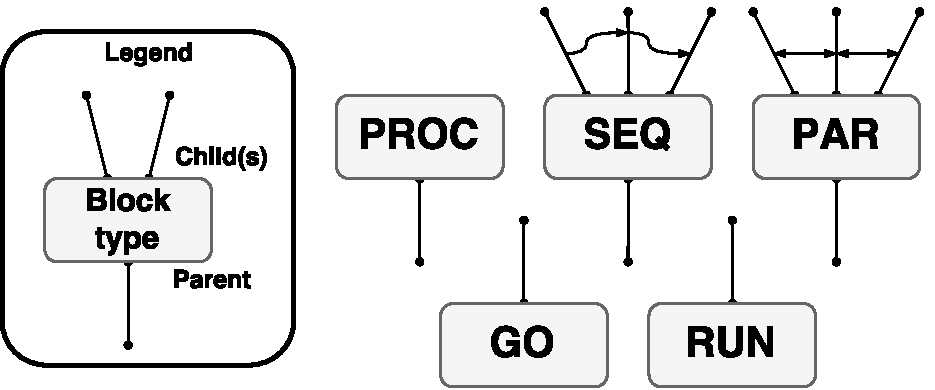
\includegraphics[width=0.8\linewidth]{fig/csp}
    \caption{Building blocks for composite processes}
    \label{fig:composite_blocks}
\end{figure}

\FloatBarrier

The combination of these building blocks can form any type of composite process. What is important to take away from this is that a composite process must \underline{\smash{always}} contain one, and only one, root node of either \texttt{GO} or \texttt{RUN}, and \underline{\smash{always}} contain one\hyp{}or\hyp{}more leaf nodes of \texttt{PROC}. 

Branch nodes, \texttt{SEQ} or \texttt{PAR}, with only one child does not alter the composite process behaviour. This becomes evident when we define a composite process of only one \texttt{PROC}, where it does not matter if multiple branch nodes of \texttt{SEQ} or \texttt{PAR} are present. This means branch nodes with one child are optional and redundant. See Figure \ref{fig:composite_axiom} for reference. 

\FloatBarrier

\begin{figure}[h]
    \centering
    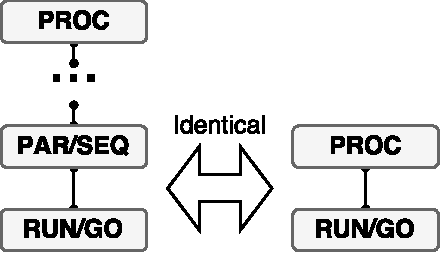
\includegraphics[width=0.5\linewidth]{fig/composite_axiom}
    \caption{Redundancy of branch nodes with one child}
    \label{fig:composite_axiom}
\end{figure}

\FloatBarrier

A composite process with a single process does not need a branch node, however a composite process with two\hyp{}or\hyp{}more \texttt{PROC} \underline{cannot} be expressed without at least one\hyp{}or\hyp{}more branch nodes.


%%%%%%%%%%%%%%%%%%%%%%%%%%%%%%%%%%%%%%%%
\subsection{Composite Process Execution}

When a process defines a composite process, the run\hyp{}time system parses and creates a composite process tree. The running process is marked as the root process of the composite process tree. The composite process tree is then traversed by the run\hyp{}time system, described by the pseudo\hyp{}code in Listing \ref{lst:algo_composite_process_tree_traversal}.

\noindent\begin{minipage}{\textwidth}
\begin{lstlisting}[style=CustomC,caption={Pseudo code for the composite process tree traversal algorithm},label={lst:algo_composite_process_tree_traversal}]
// Called with the child node of the root node
int traversal(node) {
	switch (node.type) {
	case PROC:
		process = create_process(node.fxn_and_args);
		reschedule(process);
		return Ok;
	case SEQ: // fallthrough
	case PAR:
	    if (node.num_childs < 1) return Error;
	    if (node.num_childs == 1) {
	        node.parent.this_node = node.child;
	        return traversal(node.child);
	    }
		node.childs_left = node.num_childs;
		if (node.type == SEQ) {
			return traversal(node.leftmost_child);
		} else {
		    for_each(child in node.childs) {
		    	if (traversal(child) != Ok) return Error;
		    }
		    return Ok;
		}
	}
	return Error;
}
\end{lstlisting}
\end{minipage}

After the composite process tree is traversed, all initial processes are created and added to the ready queue in the scheduler. One thing to remark about the algorithm is that process creation is lazily evaluated \citep{lazyevaluation}, which means the processes are created when needed. This is entirely the consequence of the \texttt{SEQ} block behaviour. 
Now, whether the execution type is specified to be asynchronous or synchronous, the root process continues execution or transitions process state from \textit{Ready} to \textit{Wait}, respectively. For the synchronous case, the root node transitions from \textit{Wait} to \textit{Ready} when all \texttt{PROC} in the composite process tree has ended. 

However, one also has consider the how the execution order of the composite process tree behaves when a \texttt{PROC} ends. The pseudocode in Listing \ref{lst:algo_composite_process_tree_proc_ended} shows how this is processed by the run\hyp{}time system.

\noindent\begin{minipage}{\textwidth}
\begin{lstlisting}[style=CustomC,caption={Pseudocode for the composite process tree \texttt{PROC} ended algorithm},label={lst:algo_composite_process_tree_proc_ended}]
// Called with the ended PROC
int proc_end(node) {
	while (true) {
		switch (node.type) {
		// fallthrough on GO 
		case RUN:  reschedule(node.root_process);  @\label{line:root_process_start}@
		case GO:   return Ok;
		case PROC: node = node.parent;
			       continue;
		case SEQ: // fallthrough    @\label{line:backtrack_start}@
		case PAR: if (--node.childs_left == 0) {
			          node = node.parent;
			          continue;
			      }
			      return (node.type == SEQ)
			          ? traversal(node.next_in_sequence)
				      : Ok;               @\label{line:backtrack_stop}@
		}
		return Error;
	}
}
\end{lstlisting}
\end{minipage}

The algorithm starts at the ended \texttt{PROC} and backtracks down the tree until hitting either the root node or a branch node with remaining childs left. Whenever entering a branch node, decrement the number of childs left for the given branch node. A resulting value of zero indicates all childs of the given branch has ended, and backtrack to the parent of the branch node. A resulting non\hyp{}zero value indicates there are still childs of the given branch node that are unfinished. For a \texttt{PAR} block this means the remaining childs are dispatched and will invoke the algorithm when ended. For a \texttt{SEQ} block this means there is a sequence of one\hyp{}or\hyp{}more childs remaining to be dispatched, for which the travel algorithm is called on the next child in the sequence. This is described on the lines \ref{line:backtrack_start} to \ref{line:backtrack_stop} in Listing \ref{lst:algo_composite_process_tree_proc_ended}.

The rescheduling of the root process in a synchronous composite process is described on line \ref{line:root_process_start} in Listing \ref{lst:algo_composite_process_tree_proc_ended}.


%%%%%%%%%%%%%%%%%%%%%%%%%%%%%%%%%%%%%%%%%%%%%
\subsection{Composite Process Implementation}

All relevant code for scheduler implementation are found in the following files \texttt{csp.h} and \texttt{csp.c}.

Composite processes are implemented as node trees. The challenge is how the composite tree blocks are implemented. One approach is to create a ``god'' struct for the block type, containing all data necessary for each block type. Another more modular approach is to create a struct for each composite tree block type, and one generic block type. The generic block is the interface, which is type casted to the corresponding composite tree block type. The latter approach is used in this implementation.

\noindent\begin{minipage}{\textwidth}
\begin{lstlisting}[style={CustomC},caption={Header struct type},label={lst:header_struct_type}]
typedef struct {
    enum {
        PROC_BLOCK,
        PAR_BLOCK,
        SEQ_BLOCK
    } type;
    Block *parent;
    int is_root;
    Process *root_process;
    // node tree related
    TAILQ_ENTRY(Block) node;
} Header;
\end{lstlisting}
\end{minipage}

Five structs are defined: a Header, Block, ProcBlock, ParBlock, and SeqBlock. Go and Run is not used as they are optimized away, explained later. The header struct defines the common interface between the generic block and the typed blocks. Listing \ref{lst:header_struct_type} shows the header struct. The type of the block is set in the header struct, the parent of the block, some variables for finding the root of the composite process tree, and a pointer to an optional root process. The node variable is for Block queues in \texttt{PAR} and \texttt{SEQ} blocks.

All structs Block, ProcBlock, ParBlock and SeqBlock must have the header struct as a member variable, and it must be the \underline{\smash{first}} member variable. This allows the composite process procedures and block queues to work on the generic block struct. To determine the block type, inspect the header member. Then reinterpret cast the block pointer to the correct block type through type punning. Listing \ref{lst:block_struct_type},\ref{lst:procblock_struct_type},\ref{lst:parblock_struct_type},\ref{lst:seqblock_struct_type} shows the different block types.

\noindent\begin{minipage}{.45\textwidth}
\begin{lstlisting}[caption={Generic Block struct type},style={CustomC},label={lst:block_struct_type}]
typedef struct {
    Header header;
} Block;
\end{lstlisting}
\end{minipage}\hfill
\begin{minipage}{.45\textwidth}
\begin{lstlisting}[caption={\texttt{PROC} Block struct type},style={CustomC},label={lst:procblock_struct_type}]
typedef struct {
    Header header;
    Process *process;
} ProcBlock;
\end{lstlisting}
\end{minipage}
\noindent\begin{minipage}{.45\textwidth}
\begin{lstlisting}[caption={\texttt{PAR} Block struct type},style={CustomC},label={lst:parblock_struct_type}]
typedef struct {
    Header header;
    struct {
        size_t num;
        struct BlockQ Q;
    } childs;
} ParBlock;
\end{lstlisting}
\end{minipage}\hfill
\begin{minipage}{.45\textwidth}
\begin{lstlisting}[caption={\texttt{SEQ} Block struct type},style={CustomC},label={lst:seqblock_struct_type}]
typedef struct {
    Header header;
    struct {
        size_t num;
        Block *current;
        struct BlockQ Q;
    } childs;
} SeqBlock;
\end{lstlisting}
\end{minipage}

Type punning is done through union casting. In other words, a pointer is casted to a union of the source and destination type, and reading from the destination type yields the reinterpreted pointer. This is the correct way to achieve type punning without breaking strict aliasing. A convenience macro can be made to easily achieve type punning, shown in Listing \ref{lst:type_punning}. Note that union casting and \texttt{\_\_typeof\_\_} is a GNU C extension.

\noindent\begin{minipage}{\textwidth}
\begin{lstlisting}[style={CustomC},caption={Type punning through union cast},label={lst:type_punning}]
#define BLOCK_CAST(block, destType) \
    (((union {__typeof__(block) src; destType dst;})block).dst)
\end{lstlisting}
\end{minipage}

Listing \ref{lst:type_punning_example} shows how type punning is used to convert from a generic block struct to the given typed block, and back from typed block to generic block type. This is used any time when the run\hyp{}time system either goes either way between a generic block to a typed block. 

\noindent\begin{minipage}{\textwidth}
\begin{lstlisting}[style={CustomC},caption={Type punning example},label={lst:type_punning_example}]
Block* type_punning_example(Block *block) {
    switch (block->type) {
    case PROC_BLOC: {
        ProcBlock *proc_block = BLOCK_CAST(block, ProcBlock*);
        // ... work ...
        return BLOCK_CAST(proc_block, Block*);
    }
    case PAR_BLOCK: {
        ParBlock *par_block = BLOCK_CAST(block, ParBlock*);
        // ... work ...
        return BLOCK_CAST(par_block, Block*);
    }
    case SEQ_BLOCK: {
        ProcBlock *seq_block = BLOCK_CAST(block, SeqBlock*);
        // ... work ...
        return BLOCK_CAST(seq_block, Block*);
    }
}
\end{lstlisting}
\end{minipage}

Defining a composite tree process is done through the API calls \texttt{PROC}, \texttt{PAR}, \texttt{SEQ}, \texttt{GO}, and \texttt{RUN}. The function prototypes for the API calls are shown in Listing \ref{lst:composite_process_api_prototypes}. Both \texttt{PAR} and \texttt{SEQ} has a single child block as first argument, because a non\hyp{}variadic argument must be specified before the variadic list. Also, if the variadic list is empty, the given block can be optimized away as a result of the redundancy identity shown in Figure \ref{fig:composite_axiom}.

\noindent\begin{minipage}{\textwidth}
\begin{lstlisting}[style={CustomC},caption={Composite process API prototypes},label={lst:composite_process_api_prototypes}]
Block* PROC(ProcessFxn fxn, ...);
Block* PAR(Block *first_child, ...);
Block* SEQ(Block *first_child, ...);
void GO(Block *root);
void RUN(Block *root);
\end{lstlisting}
\end{minipage}

Currently, the API calls \texttt{PROC}, \texttt{PAR} and \texttt{SEQ} allocates a typed block on the heap. \texttt{GO} or \texttt{RUN} does not however allocate any typed block on the heap. \texttt{PROC} also creates a process with the given function pointer and arguments, and sets the process pointer in the typed block to the created process. \texttt{PAR} and \texttt{SEQ}, if two or more childs given, inserts each child in the block queue and records the number of childs. \texttt{SEQ} initializes the current block pointer to the first child. 

Both API calls \texttt{GO} and \texttt{RUN} receives a root block, which the root flag of the block is set to true. \texttt{GO} traverses the resulting composite process tree, starting at the root block. When the traversal returns, the API call returns as well, and the running process continues execution. \texttt{RUN} sets the root process pointer to the running process, and traverses the resulting composite process tree, starting at the root block. When the traversal returns, the running process yields with the process state set to \textit{Wait}. The running process is resumed when the root block finishes.

The traversal implementation is very straightforward, following the pseudocode in Listing \ref{lst:algo_composite_process_tree_traversal}. Only difference is process creation happens in the API call \texttt{PROC}, rather in the traversal procedure. This has to do with the simplifications of the variadic list handling. 

The \texttt{PROC} ended implementation follows the pseudocode in Listing \ref{lst:algo_composite_process_tree_proc_ended} with some slight modifications. The \texttt{RUN} and \texttt{GO} cases are removed, as they are simplified to a root flag. Whenever either \texttt{PROC}, \texttt{SEQ} or \texttt{PAR} block, a \texttt{block\_done} variable is set to true. This is checked at the end of the switch case, and if the current block is the root block, the root process is rescheduled if the composite tree is synchronous. 

An added cleanup procedure must be called when the root block finishes, as the entire tree is allocated on the heap. This is a simple tree traversal, freeing up each block in a post\hyp{}order fashion. 


%%%%%%%%%%%%%%%%%%%%%%%%%%%%%%%%%%%%%%%%%%%%%%%%%%%%%%%%%%%%%%%%%%%%%%%%%%%%%%%%%%%%%%%%%%%%%%
\section{Timers}
\label{sec:timers}

Timers are used to suspend a process for a given amount of time. This is used in two situations: in a normal process execution, or in an alternation process. 

In a normal process execution, whenever a timeout is specified, the process is suspended. The run\hyp{}time system places the process in the sleep tree based on the specified timeout period. The process is resumed by the run\hyp{}time system when the timeout period is expired.

In an alternation process, the timeout is specified as a guarded alternative. When the alternative is activated, the alternation process is placed in the alternation sleep tree based on the specified timeout period. One of two things happens: either the timeout period is expired and the run\hyp{}time system registers the timeout alternative in the alternation available set. If the alternation process is still suspended, resume it. Or, the alternation process is resumed before the timeout expiration, and the timeout alternative is deactivated, removing it from the alternation sleep tree. 


%%%%%%%%%%%%%%%%%%%%%%%%%%%%%%%%%
\subsection{Timer Implementation}

Timers is realized through the sleep trees in the scheduler. Invoking a timer on a process is done through the API call \texttt{SLEEP}, which takes an expiration time in microseconds as argument. If the expiration time is zero, the process yields with no additional changes. If non\hyp{}zero, the process registers the expiration time in the process struct, and adds itself to the sleep tree in the scheduler. Then, yielding with the state \textit{Sleep}. When the time expires, the scheduler will reschedule the sleeping process.

For alternation constructs, the timeout guard registers the process in the alternation sleep tree. The same functionality applies here for normal timers. However, if the alternation construct completes the selection process before the timeout occurs, the alternation process removes itself from the alternation sleep tree. 


%%%%%%%%%%%%%%%%%%%%%%%%%%%%%%%%%%%%%%%%%%%%%%%%%%%%%%%%%%%%%%%%%%%%%%%%%%%%%%%%%%%%%%%%%%%%%%
\section{Channels}
\label{sec:channels}

Channels forms the means of interprocess communication and synchronization, following the message passing model. There are mainly three aspects of channel design that must be considered, namely synchronous or asynchronous communication, channel disjointness, and type\hyp{}safe data transfer. 


%%%%%%%%%%%%%%%%%%%%%%%%%%%%%%%%%%%%%%%%%%%%%%%%%%%%%%%%%%%%%%%%%%%%%
\subsection{Synchronous and Unbuffered, or Asynchronous and Buffered}

Coming from the CSP model, channels are implemented as unbuffered and synchronous, and are sometimes called a synchronous rendezvous. This is used as a one\hyp{}way transfer of data between a receiver and a sender. Both the receiver and sender must be available on the channel for the transfer to occur. If one of the ends are not present, the other end must wait until both ends are ``ready''.

The channel design follows the CSP model, being unbuffered and synchronous.


%%%%%%%%%%%%%%%%%%%%%%%%%%%%%%%%%
\subsection{Channel Disjointness}

Some channels have a notion of disjointness \citep[see][chapter 3.3.1]{xc}, setting restrictions on how many processes are allowed to use a channel, and how many unique senders or receivers a channel can have. These designs are often denoted as a one\hyp{}to\hyp{}one, any\hyp{}to\hyp{}one, one\hyp{}to\hyp{}any, or any\hyp{}to\hyp{}any channels, following the \textit{\#Senders}\hyp{}to\hyp{}\textit{\#Receivers} scheme.

Creating four version of the channel design, one for each of the four combinations of \textit{one} and \textit{any}, might turn out to be a flexible approach. This allows the programmer to handpick the channel type for certain use cases, i.e.  one\hyp{}to\hyp{}any for multiple readers and one writer, etc.. 

One might argue ``Why not just have a any\hyp{}to\hyp{}any design, and cover all use cases?''. Enforcing disjointness increases the expressiveness of the abstraction, allowing the programmer to create more correct programs that reflects a truer behaviour of the system. As well, this also gives the implementation some assumptions allowing better optimizations for each design. 

However, for the sake of simplicity and as a result of the limitations of C, only the any\hyp{}to\hyp{}any version will be implemented. 


%%%%%%%%%%%%%%%%%%%%%%%%%%%%%
\subsection{Type\hyp{}Safety}

Channels are also used to transfer data between processes. Type errors can be an issue in a data transfer, where the type of data sent over a channel does not match the type of data expected to be received. 

An example can be a sender and a receiver on a channel with no type\hyp{}safety. Sender sends a message of type A, which has a 4 byte size representation. Receiver B expects to receive a message of type B, which has a 2 byte size representation, and allocates the appropriate memory. When the transfer of data occurs, the channel writes the 4 bytes of data to the memory allocated only for 2 bytes. 2 bytes are written past the allocated memory, and memory corruption has occurred. See illustration in Figure \ref{fig:type_error} for reference. This illustrates the dangers of not enforcing type\hyp{}safety on channels. 

\FloatBarrier

\begin{figure}[h]
    \centering
    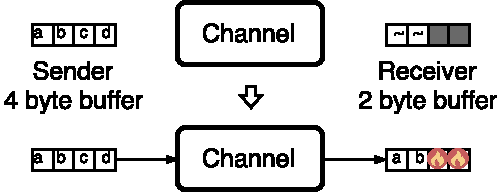
\includegraphics[width=0.6\linewidth]{fig/type_error}
    \caption{Memory corruption from conflicting types between sender and receiver}
    \label{fig:type_error}
\end{figure}

\FloatBarrier

Type\hyp{}safe channels enforces only transfer of messages of only one type. This in turn enforces the sender and receiver to agree on the type of the message. This should be favorable, as type errors should be treated as bugs in a program. Channels should therefore be as type\hyp{}safe as possible.

C is however known for not being very type\hyp{}safe. The language enforces type\hyp{}safety to some degree, but is easily circumventable through type casting to pointer types. A common source of type errors in C programs are pointers casted from and to void pointers, \texttt{void*}. Void pointers are used for memory with an unspecified type, which are convenient for implementation of generic interfaces. This is most likely how channels will implement data transfer, being compatible with any type. Knowing this, complete type\hyp{}safe channels in C will be impossible without code bloat and breaking encapsulation\footnote{This is possible, but requires heavy use of macros and leaking implementation details to the programmer}. A compromise is size\hyp{}safe channels. Instead of ensuring the type matches, the size representation of the type must match on both sides. This should not require much overhead, and at least avoids memory corruption, illustrated in Figure \ref{fig:type_error}.


%%%%%%%%%%%%%%%%%%%%%%%%%%%
\subsection{Channel Implementation}

All relevant code for channel implementation are found in the following files \texttt{chan.h} and \texttt{chan.c}.

This channel implementation implements a synchronous, unbuffered, size\hyp{}safe channels. However, disjointed channels proved to be to difficult to implement, which is why only any\hyp{}to\hyp{}any channels are used. This is explained more later. 

Channels is realized by a channel struct and a channel end struct. A channel struct represents a created channel, while a channel end represents a process waiting on a channel. The two struct are shown in Listing \ref{lst:channel_type_struct} and \ref{lst:channel_end_type_struct}.

\noindent\begin{minipage}{.45\textwidth}
\begin{lstlisting}[caption={Channel type struct},style={CustomC},label={lst:channel_type_struct}]
typedef struct {
    size_t data_size;
    struct ChanEndQ endQ;
    struct ChanEndQ altQ;
} Chan;
\end{lstlisting}
\end{minipage}\hfill
\begin{minipage}{.45\textwidth}
\begin{lstlisting}[caption={Channel end type struct},style={CustomC},label={lst:channel_end_type_struct}]
typedef struct {
    enum {
        CHAN_WRITER,
        CHAN_READER,
        CHAN_ALTER,
    } type;
    void *data;
    Chan *chan;
    Process *process;
    AltGuard *guard;
    TAILQ_ENTRY(ChanEnd) node;
} ChanEnd;
\end{lstlisting}
\end{minipage}

The channel constructor is called \texttt{chan\_create}, and takes the size of the data type as an argument. The channel struct is allocated on the heap. The data size is stored, and the two channel end queues are initialized. The API call \texttt{CHOPEN} calls the channel constructor and returns the channel struct pointer. 

The channel destructor is called \texttt{chan\_free}, and frees the channel struct. The API call \texttt{CHCLOSE} calls the channel destructor.

The channel struct contains two channel end queues, called hereafter end queue and altend queue. These queues are used when processes has to wait on a channel for a process to be available on the other end. Two queues are used instead of one, as alternation waiting is separated from normal waiting. The end queue can contain both writers and readers, but not at the same time. The altend queue only contains alternation processes trying to read the channel. 

Three operations can be done on a channel struct: channel write, channel read and channel alternation read. All these three operations take a channel struct pointer, a data pointer, and the size of the data as arguments. There are as well two additional internal operations for alternation, namely alternation enabling and disabling of a channel. 

A channel read does the following: the channel end queue of the channel is checked. If the queue is non\hyp{}empty and contains writers, the first channel end is popped from the end queue. The data transfer is completed, and the writer process is rescheduled. The reading process resumes execution. If the end queue is empty or contains readers, a channel end struct is allocated on the stack and initialized. The channel end is inserted at the end of the end queue of the channel, and the reader process yields with the state \textit{Wait}. When the process is resumed, the channel operation is already completed. The API call \texttt{CHREAD} calls the channel read operation, and returns whether the write was successful or not. 

A channel write does the following: the altend queue is checked before the end queue. If it contains an alternation process, the writer tries to accept the alternation alternative. If it is accepted, the data transfer is completed, and the alternation process is rescheduled. If this fails, the end queue is checked. If it is non\hyp{}empty and contains readers, the first channel end is popped from the end queue. The data transfer is completed, and the reader process is rescheduled. The writer process resumes execution. If the end queue is empty or contains writers, a channel end struct is allocated on the stack and initialized. The channel end is inserted at the end of the end queue of the channel, and the reader process yields with the state \textit{Wait}. When the process is resumed, the channel operation is already completed. The API call \texttt{CHWRITE} calls the channel write operation, and returns whether the write was successful or not. 

A channel alternation read consists of multiple stages. First, the alternation process enables the channel for alternation synchronization. The end queue is checked, and if it contains writers, the channel is marked as available. If empty or contains readers, the alternation process is inserted in the altend queue. The case where the channel is available, the alternation process completes the data transfer with the channel alternation read operation. This pops the first writer from the end queue, the data transfer is completed, and the waiting writer process is rescheduled. Lastly, regardless if the alternation process or a writer process completed the channel operation, the alternation process disables the channel for alternation synchronization. This removes the channel end from the altend queue. The channel alternation read operation is done internally by the run\hyp{}time system.

Transfer of data is optimized depending on the data size. If the data size is either 1, 2, 4, or 8 bytes, data is transferred as integer assignments. If data size is zero, nothing happens. Every other data size is transferred with a normal \texttt{memcpy} call. See Listing \ref{lst:channel_data_transfer} on how this is done.

\noindent\begin{minipage}{\linewidth}
\begin{lstlisting}[caption={Channel data transfer},style={CustomC},label={lst:channel_data_transfer}]
void channel_datatransfer(void *dst, void *src, size_t size) {
    switch (size) {
    case 0:    /* do nothing */                   break;
    case 1:   *(uint8_t *)dst =  *(uint8_t *)src; break;
    case 2:  *(uint16_t *)dst = *(uint16_t *)src; break;
    case 4:  *(uint32_t *)dst = *(uint32_t *)src; break;
    case 8:  *(uint64_t *)dst = *(uint64_t *)src; break;
    default: memcpy(dst, src, size); break;
    }
}
\end{lstlisting}
\end{minipage}

This implementation only implements an any\hyp{}to\hyp{}any channel. Implementing one\hyp{}to\hyp{}one, any\hyp{}to\hyp{}one, or one\hyp{}to\hyp{}any channels proved to be too difficult. There was no possibility of enforcing this during compile\hyp{}time, as C lacks the language features for this. Run\hyp{}time checks was possible, but created too much overhead and was too error\hyp{}prone to be any useful. So for the sake of code simplicity, only implementing an any\hyp{}to\hyp{}any channel was favored. 


%%%%%%%%%%%%%%%%%%%%%%%%%%%%%%%%%%%%%%%%%%%%%%%%%%%%%%%%%%%%%%%%%%%%%%%%%%%%%%%%%%%%%%%%%%%%%%%%%%%
\section{Alternation}

Alternation is used to wait on multiple alternatives, selecting only one available alternative to execute. Each alternative can be supplemented with a corresponding code execution. Optionally, alternatives are guarded by a boolean condition, which are evaluated at the initialization of the alternation process. Only alternatives for which the guard condition is true is enabled for selection. Alternatives consists of the following: channel reads, timeouts and skip. The alternation process is a synchronous process, meaning the alternating process is waiting until an alternative is available and selected. 

Alternation is used together with the switch construct in C. Alternation takes in a set of ordered, alternatives, and returns the number, hereafter called key, corresponding to the alternative that was selected. Keys are incrementally ordered, starting at zero on the first alternative. When an alternative is selected and a key is returned, the operation corresponding to the alternative is already executed and branches to the matching switch case. 

Listing \ref{lst:alternation_setup} displays pseudocode of the alternation setup, with three guarded alternatives of the three possible alternatives. Note that the code section for each guard is optional, and can be completely left out.

\noindent\begin{minipage}{\textwidth}
\begin{lstlisting}[style=CustomC,caption={Pseudocode of alternation setup},label={lst:alternation_setup}]
switch (Alternation(
	Guard(condition,  // Guard 0, enabled when `condition` is true
		ChanRead(chan, data, sizeof(data)),
	Guard(true,       // Guard 1, always enabled
		Timeout(time)),
	Guard(false,      // Guard 2, never enabled
		Skip())
)) {
case 0: // Code for Guard 0
case 1: // Code for Guard 1
case 2: // Code for Guard 2
}
\end{lstlisting}
\end{minipage}


%%%%%%%%%%%%%%%%%%%%%%%%%%%%%%%%%%%%%%%
\subsection{Alternation Process Stages}
\label{subsec:alternation_process_stages}

The alternation process consists of three stages: activation, selection, and deactivation. It has one set of available alternatives, initialized to empty. Key is initialized to 0.

The first stage, activation, checks if the guards are enabled and the corresponding alternatives are available. First, iterating over every guard and checking the guard condition. If the condition is true, the alternative is activated. The alternative is also given a corresponding key. If condition is false, the alternative is ignored. The key is incremented for each check regardless if activated or not. This is to match each guards with the case numbers. When an alternative is activated, it is checked if available. If available, it is registered in the set of available alternatives.

The second stage, selection, selects which alternative to synchronize on from the set of available alternatives. After the first stage, one of two cases apply: either some alternatives were already available during activation, or non were. In other words, the set of available alternatives is either non\hyp{}empty or empty. If non\hyp{}empty, an alternative is selected and moves on to the third stage. If empty, the alternation process is suspended and waits for an alternative to be available. When the alternation process is resumed, the set of available alternative is now populated by one or more alternatives. An alternative is selected and moves on to the third stage. More details about selection in Section \ref{subsec:alternation_fairness}.

In the third stage, deactivation, every alternative is iterated over and deactivated if the guard conditional is true.


%%%%%%%%%%%%%%%%%%%%%%%%%%%
\subsection{Alternatives}

The three alternatives, when enabled, operates as follows:

\begin{itemize}[topsep=0em,itemsep=-1em,partopsep=0.5em,parsep=1em]
    \item \textbf{Channel Read}: specifies a channel read on a given channel, and stores the message in a given variable. The alternative is available when a sender is on the channel. 
    
    \item \textbf{Timeout}: specifies a timeout for the selection process. If the alternation process has not selected an alternative within the specified time, the timeout guard is selected and the alternating process is resumed. 
    
    \item \textbf{Skip}: is always available. In other words, if no other alternatives are available at the alternation initialization, the skip alternative is automatically selected. 
\end{itemize}

It might be tempting to suggest that a skip alternative makes the alternation process asynch\-ronous, but this is not the case. Whenever the alternation selects the skip alternative as a result of no other available alternatives, it simply synchronizes on the skip alternative. 

Alternation can consist of multiple enabled channel read alternatives. Only one enabled timeout and skip alternative will be registered. If multiple timeout alternatives are enabled, the timeout alternative with the smallest expiration time will be used. If multiple skip alternatives are enabled, the first skip alternative will be used. 

An alternative is initially deactivated. During the alternation process, if the condition of the guard is true, the alternative is activated. Activating an alternative registers the alternation process' interest in synchronizing with the alternative. Deactivating an alternative unregisters this interest. 

An alternative which is not available when activated has the added responsibility of resuming the alternation process when becoming available. It should only resume the alternation process if it is still suspended, as multiple alternatives might become available before the alternation resumes execution.


%%%%%%%%%%%%%%%%%%%%%%%%%%%%
\subsection{Alternative Selection}
\label{subsec:alternative_selection}

During the selection stage the set of available alternatives are populated with one or more members. The following algorithm chooses an alternative from that set:

\begin{enumerate}[topsep=0em,itemsep=-1em,partopsep=0.5em,parsep=1em]
    \item If set only contains one alternative, choose that alternative and goto \ref{line:alt_choose}.
    \item If the set contains a skip alternative, remove it from the set.
    \item Uniform pesudo\hyp{}randomly choose one alternative from the remaining set. 
    \item Complete the associated action with the alternative. \label{line:alt_choose}
    \item Return the key from the chosen alternative.
\end{enumerate}

If the selected alternative is a channel read, the data transfer completes and both processes on each end resumes. If the selected alternative is a timeout or skip, no additional actions are made and the alternation process continues. 


%%%%%%%%%%%%%%%%%%%%%%%%%%%%%%%%%%%%%
\subsection{Fairness and Determinism}
\label{subsec:alternation_fairness}

The use of a pseudo\hyp{}random choice of multiple available alternatives makes it fair and non\hyp{}deterministic. The reasoning for this policy being fair is subtle. If it was not fair, starvation would occur when arbitrating between multiple available alternatives. This is however only possible within finite amount of time, as the arbitration is uniform pseudo\hyp{}random. Eventually, all alternatives will be chosen. This is the same design and reasoning the Go programming language uses \citep[see][Select statements]{golangspec}.

This does make the choice non\hyp{}deterministic, as it is a pseudo\hyp{}random choice. The discussion between fairness and determinism is an age old debate within the concurrent system design, and for all practical reasons the alternation construct favors fairness over determinism. 


%%%%%%%%%%%%%%%%%%%%%%%%%%%%%%%%%%%%%%%
\subsection{Alternation Implementation}

All relevant code for channel implementation are found in the following files \texttt{alt.h} and \texttt{alt.c}.

Alternation is realized by an alternation struct for the alternation process, and a guard struct for each guarded alternative. Listing \ref{lst:alt_type_struct} and \ref{lst:guard_type_struct} shows the struct definition for the alternation type and guard type, respectively. 

The alternation constructor is called \texttt{alternation\_init}, and takes a pre\hyp{}allocated alternation struct as argument. The alternation struct is allocated on the stack. The constructor initializes the struct members and the guard queue, and saves the running process pointer. This is used to reschedule the alternation process if it suspends itself waiting. 

The alternation destructor is called \texttt{alternation\_cleanup}, and takes an alternation struct as argument. It iterates over the guard queue, calling the guard destructor for each guard. The available guard array is freed as well, as it is allocated on the heap. 

\noindent\begin{minipage}{.45\textwidth}
\begin{lstlisting}[caption={Alternation type struct},style={CustomC},label={lst:alt_type_struct}]
typedef struct {
    int key_count;
    int is_accepted;
    Guard *winner;
    struct {
        int num;
        Guard **guards;
    } ready;
    struct {
        size_t num;
        struct GuardQ Q;
    } guards;
    // skip and time guards 
    // only exists one of
    Guard *guard_skip; 
    Guard *guard_time;
    // alternation process
    Process *process;
} Alternation;
\end{lstlisting}
\end{minipage}\hfill
\begin{minipage}{.45\textwidth}
\begin{lstlisting}[caption={Guard type struct},style={CustomC},label={lst:guard_type_struct}]
typedef struct {
    enum {
        GUARD_SKIP,
        GUARD_TIME,
        GUARD_CHAN
    } type;
    int key;
    Alternation *alternation;
    TAILQ_ENTRY(Guard) Qnode;
    RB_ENTRY(Guard) RBnode;
    // Timer Guard
    uint64_t  usec;
    // Chan Guard
    Chan *chan;
    ChanEnd ch_end;
    struct {
        void *ptr;
        size_t size;
    } data;
    int in_chan;
} Guard;
\end{lstlisting}
\end{minipage}

The guard constructor is called \texttt{alternation\_guardcreate}, and is used for all of the three types of guards. The guard struct is allocated on the heap. It takes a guard type, expiration time in microseconds, channel struct pointer, data pointer, and the size of the data. The API call \texttt{CHAN\_GUARD} calls the constructor with the \texttt{GUARD\_CHAN} type and the channel related arguments. Note that the channel end struct is allocated alongside the guard struct. The API call \texttt{TIME\_GUARD} calls the constructor with the \texttt{GUARD\_TIME} type and the expiration time. Lastly, the API call \texttt{SKIP\_GUARD} calls the constructor with only the \texttt{GUARD\_SKIP} type. 

The guard destructor is called \texttt{alternation\_guardfree}, and frees the guard struct.

The alternation process starts with defining different guards with the following API calls \texttt{SKIP\_GUARD}, \texttt{TIME\_GUARD} and \texttt{CHAN\_GUARD}. Each call evaluates the boolean condition supplied as argument. If true, calls the corresponding guard constructor and returns the guard struct pointer. If false, a \texttt{NULL} pointer is returned. 

The list of guards is stored as a variadic list and sent as arguments to the API call \texttt{ALT}. The alternation struct is allocated on the stack, and initialized with the alternation constructor. Then, the variadic list is iterated over, adding each guard to the alternation struct. A \texttt{NULL} pointer guard is skipped, but the key value is incremented regardless. After evaluating and adding each guard, the selection procedure is called. Following the alternative selection algorithm in Section \ref{subsec:alternative_selection}, some slight additions are used. The available guards array is allocated as an guard struct pointer array, equal to the number of enabled guards. This is dynamically allocated on the heap. The chosen guard is stored in the \texttt{winner} member in the alternation struct. For the uniform pseduo\hyp{}random function, the library function \texttt{rand} is used.

